\documentclass[11pt,a4paper]{article}
\usepackage[utf8]{inputenc}
\usepackage[portuguese]{babel}
\usepackage{amsmath}
\usepackage{amsfonts}
\usepackage{amssymb}
\usepackage{graphicx}
\usepackage{booktabs}
\usepackage{geometry}
\usepackage{hyperref}
\usepackage{float}

\geometry{margin=25mm}

\title{Estudo Científico: Dimensionamento de Balões de Hélio para Sustentação Humana}
\author{Relatório Técnico Automatizado}
\date{12 de Junho de 2026}

\begin{document}
	
	\maketitle
	
	\begin{abstract}
		Este documento apresenta uma análise física e matemática detalhada sobre o volume, diâmetro e quantidade de balões de hélio necessários para colocar uma pessoa em suspensão no ar. O estudo fundamenta-se no Princípio de Arquimedes e nas propriedades termodinâmicas dos gases sob Condições Normais de Temperatura e Pressão (CNTP).
	\end{abstract}
	
	\section{Introdução e Fundamentos Teóricos}
	Para que um corpo permaneça suspenso na atmosfera terrestre, a força resultante vertical deve ser nula. O princípio físico que rege este fenómeno é o \textbf{Princípio de Arquimedes}, que dita que qualquer corpo imerso num fluido sofre uma força de empuxo ($F_E$) vertical e para cima, igual ao peso do fluido deslocado.
	
	A condição elementar de equilíbrio estático é dada por:
	\begin{equation}
		F_E = P_{\text{total}}
	\end{equation}
	
	Onde o peso total ($P_{\text{total}}$) engloba a massa da pessoa ($m_p$), a massa do gás hélio ($m_{\text{he}}$), a massa do invólucro dos balões ($m_{\text{balão}}$) e os elementos de fixação ($m_{\text{cabos}}$), multiplicados pela aceleração da gravidade ($g$):
	\begin{equation}
		P_{\text{total}} = (m_p + m_{\text{he}} + m_{\text{balão}} + m_{\text{cabos}}) \cdot g
	\end{equation}
	
	\section{Dados de Referência (CNTP)}
	Para efeitos de modelação, assumem-se os seguintes parâmetros padrão ao nível do mar e a aproximadamente $20^\circ\text{C}$:
	\begin{itemize}
		\item \textbf{Massa de referência da pessoa ($m_p$):} $70\text{ kg}$
		\item \textbf{Densidade do ar atmosférico ($\rho_{\text{ar}}$):} $\approx 1,20\text{ kg/m}^3$
		\item \textbf{Densidade do gás hélio ($\rho_{\text{he}}$):} $\approx 0,18\text{ kg/m}^3$
	\end{itemize}
	
	\section{Cálculo da Capacidade de Sustentação}
	A força líquida de ascensão por unidade de volume ($1\text{ m}^3$) de hélio é determinada pela diferença de densidade entre o meio fluido (ar) e o gás interno (hélio):
	\begin{equation}
		\Delta\rho = \rho_{\text{ar}} - \rho_{\text{he}}
	\end{equation}
	\begin{equation}
		\Delta\rho = 1,20\text{ kg/m}^3 - 0,18\text{ kg/m}^3 = 1,02\text{ kg/m}^3
	\end{equation}
	
	Isto significa que, teoricamente, cada metro cúbico ($1000\text{ litros}$) de hélio puro possui a capacidade de erguer uma massa líquida de $\mathbf{1,02\text{ kg}}$.
	
	\section{Determinação do Volume Total Necessário}
	Para suspender a massa padrão de $70\text{ kg}$:
	\begin{equation}
		V_{\text{teórico}} = \frac{m_p}{\Delta\rho} = \frac{70\text{ kg}}{1,02\text{ kg/m}^3} \approx 68,63\text{ m}^3
	\end{equation}
	
	Considerando as massas adicionais desprezadas na idealização (peso do látex, cordas, arnês) e aplicando uma margem de segurança operacional para garantir a flutuabilidade positiva, adota-se um volume prático de:
	\begin{equation}
		V_{\text{total}} \approx 75\text{ m}^3
	\end{equation}
	
	\begin{figure}[H]
		\centering
		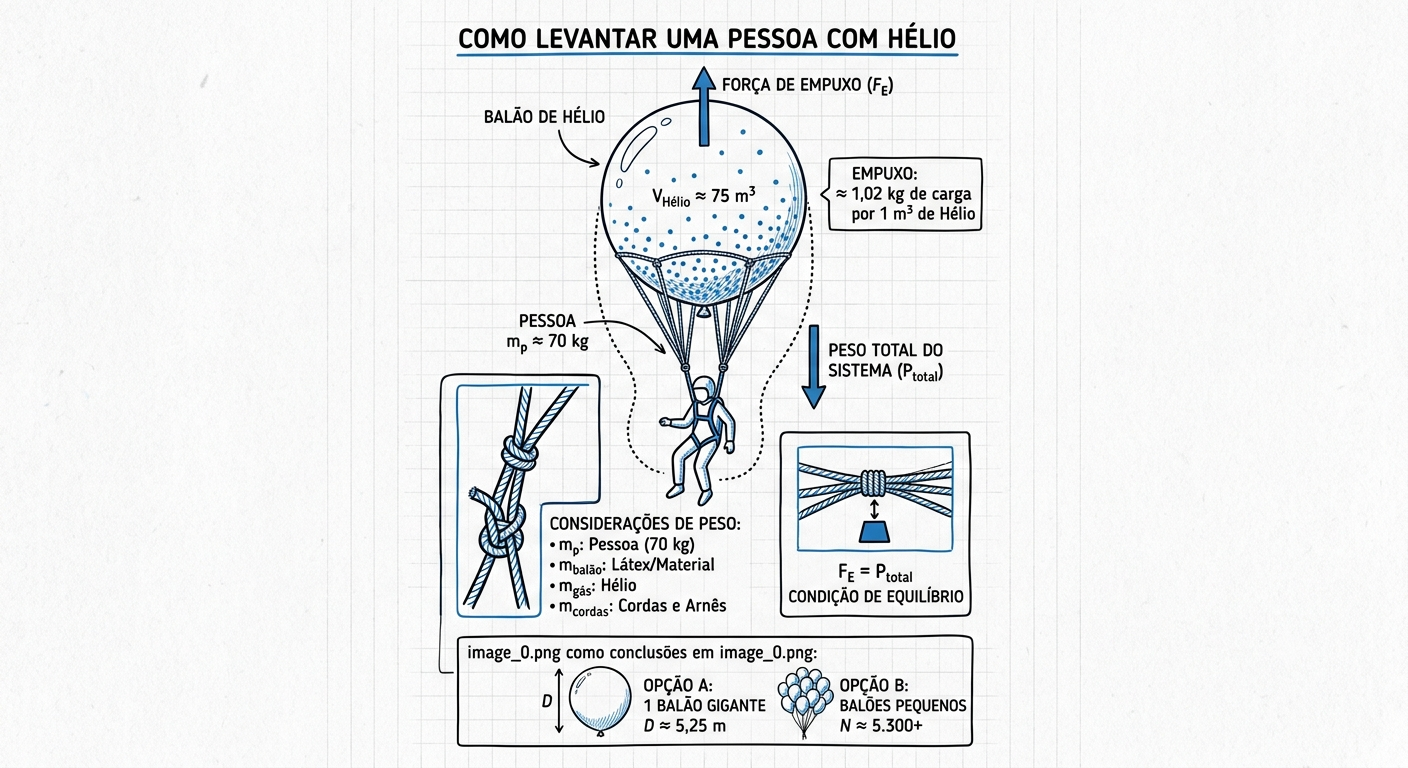
\includegraphics[width=\textwidth]{fig1}
	\end{figure}
	
	\section{Análise de Cenários de Configuração}
	
	\subsection{Cenário A: Balão Esférico Único}
	Assumindo a geometria de uma esfera perfeita, o volume é definido por:
	\begin{equation}
		V = \frac{4}{3}\pi r^3
	\end{equation}
	
	Substituindo o volume prático necessário ($V = 75\text{ m}^3$):
	\begin{equation}
		75 = \frac{4}{3}\pi r^3 \implies r^3 = \frac{225}{4\pi} \approx 17,9049
	\end{equation}
	\begin{equation}
		r = \sqrt[3]{17,9049} \approx 2,616\text{ metros}
	\end{equation}
	
	Sendo o diâmetro ($D$) o dobro do raio ($r$):
	\begin{equation}
		D = 2 \times 2,616 \approx \mathbf{5,23\text{ metros}}
	\end{equation}
	
	\subsection{Cenário B: Balões de Festa Convencionais}
	Para balões comerciais com um diâmetro unitário de $30\text{ cm}$ ($D = 0,30\text{ m} \implies r = 0,15\text{ m}$):
	\begin{equation}
		V_{\text{balão}} = \frac{4}{3}\pi (0,15)^3 \approx 0,01414\text{ m}^3
	\end{equation}
	
	Dividindo o volume total pelo volume unitário:
	\begin{equation}
		N_{\text{teórico}} = \frac{75\text{ m}^3}{0,01414\text{ m}^3} \approx 5304\text{ balões}
	\end{equation}
	
	\textbf{Nota Prática:} Na realidade física, o acúmulo de peso de 5300 nós e fios exige um ajuste empírico, elevando a necessidade real para a faixa de \textbf{6.000 a 6.500 balões}.
	
	\section{Modelagem da Relação Peso vs Diâmetro}
	A função matemática que descreve o diâmetro mínimo do balão único ($D$) em metros em função da massa da pessoa ($m_p$) em quilogramas, incluindo a correção proporcional de margem de segurança, é expressa por:
	\begin{equation}
		D(m_p) = 2 \cdot \sqrt[3]{\frac{3 \cdot (m_p \cdot 1,071)}{4\pi \cdot 1,02}}
	\end{equation}
	
	A Tabela~\ref{tab:valores} sintetiza os pontos notáveis desta função:
	
	\begin{table}[h]
		\centering
		\caption{Diâmetro e Volume do Balão Único em Função do Peso}
		\label{tab:valores}
		\begin{tabular}{ccc}
			\toprule
			\textbf{Peso da Pessoa ($m_p$)} & \textbf{Volume Requerido ($V$)} & \textbf{Diâmetro Mínimo ($D$)} \\ \midrule
			50 kg  & $\approx 53,5\text{ m}^3$  & $\approx 4,67\text{ m}$ \\
			70 kg  & $\approx 75,0\text{ m}^3$  & $\approx 5,24\text{ m}$ \\
			90 kg  & $\approx 96,5\text{ m}^3$  & $\approx 5,70\text{ m}$ \\
			110 kg & $\approx 118,0\text{ m}^3$ & $\approx 6,10\text{ m}$ \\ \bottomrule
		\end{tabular}
	\end{table}
	
	O gráfico \ref{graf1} que mostra a relação entre o peso da pessoa (em kg) e o diâmetro necessário para um único balão gigante (em metros).
	
	Repare que a curva não é uma linha reta: como o volume de uma esfera cresce com o cubo do raio ($V \propto r^3$), o diâmetro aumenta de forma mais rápida no início e depois começa a suavizar para pesos maiores.
	
	A fórmula matemática exata que gera este gráfico (já incluindo a margem de segurança para cabos e o invólucro do balão que usamos nos cálculos anteriores) é:
	
	$$D(m_p) = 2 \times \sqrt[3]{\frac{3 \times (m_p \times 1,071)}{4 \pi \times 1,02}}$$
	
	\begin{figure}[H]
		\centering
		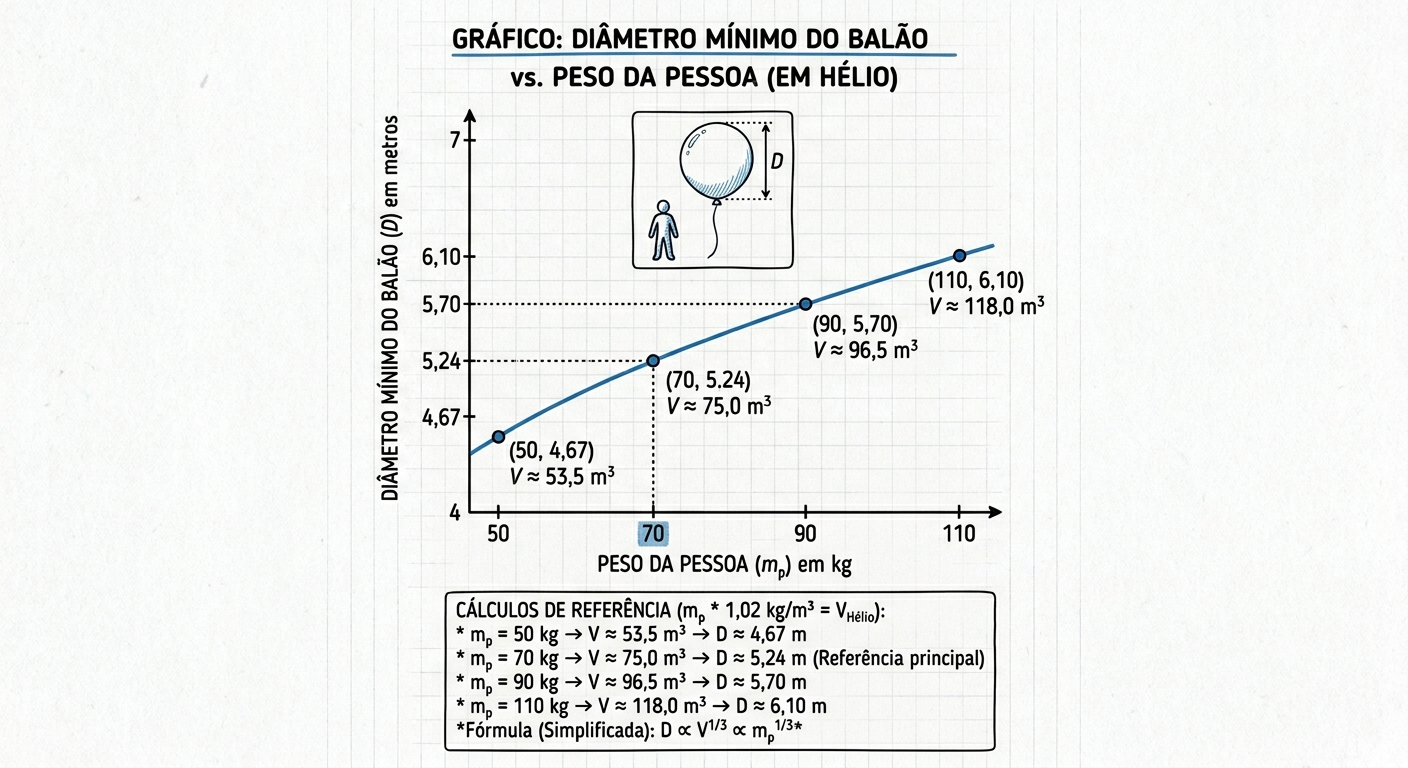
\includegraphics[width=\textwidth]{fig2}
		\label{graf1}
	\end{figure}
	
	\section{Referências Bibliográficas}
	\begin{enumerate}
		\item HALLIDAY, D.; RESNICK, R.; WALKER, J. \textit{Fundamentos de Física Volume 2: Gravitação, Ondas e Termodinâmica}. Rio de Janeiro: LTC.
		\item LIDE, D. R. \textit{CRC Handbook of Chemistry and Physics}. 84th Edition. CRC Press, 2003.
		\item TRAPPE, Jonathan. \textit{Cluster Ballooning Flight Records and Technical Data} (Casos práticos de estudo de balonismo de agrupamento).
	\end{enumerate}
	
\end{document}